%!TEX output_directory = .aux
%!TEX copy_output_on_build(true)

\documentclass[11pt,a4paper, titlepage]{article}
\usepackage[a4paper, total={6.5in, 8in}]{geometry}
\usepackage[utf8]{inputenc}
\usepackage{amsfonts}
\usepackage{amssymb}
\usepackage{amsmath}
\usepackage{mathtools}
\usepackage{forest}
\usetikzlibrary{shapes.geometric,positioning, arrows, trees, positioning, fit, calc}
\usepackage{amsthm}

\title{An Analysis of smart voting in liquid democracy}
\author{Giannis Tyrovolas}
\date{\today}
\newtheorem{theorem}{Theorem}[section]
\newtheorem{prop}[theorem]{Proposition}
\newtheorem*{remark}{Remark}
\DeclarePairedDelimiter\abs{\lvert}{\rvert}
\DeclarePairedDelimiter\norm{\lVert}{\rVert}


\theoremstyle{definition}
\newtheorem{definition}[theorem]{Definition}
\newtheorem{example}[theorem]{Example}
\newtheorem{corollary}[theorem]{Corollary}
\newtheorem{lemma}[theorem]{Lemma}
\newtheorem{proposition}[theorem]{Proposition}
\newtheorem*{idea}{Idea}
\let\vec\mathbf

\begin{document}

\maketitle

\tableofcontents

\newpage

\section{Preliminaries}

\subsection{Ballots}


An election consists of a finite set of voters, voting on a finite set of issues. For each issue there is a finite set of alternatives. A special alternative is the abstention represented by $*$. Finally, there is an aggregation function that decides what the result of the election is. Formally:

\begin{definition}[Election]
    An \emph{election} consists of a tuple $\langle N, I, D, \mathcal{G}\rangle $ where $N = \{1,..., n\} $ is a finite non-empty set. The finite non-empty set $I$ holds represents the issues of the election. For each $i \in I$, $D(i)$ is a finite non-empty set. The function $\mathcal{G}$ is an aggregation function that inputs the votes on every voter on every issue and outputs the resulting vote of the group on each issue.
\end{definition}

For single-issue elections we omit the reference to $I$ and abbreviate $D(i)$ to $D$. So, that function $\mathcal{G}$ is $\mathcal{G} \colon D^N \longrightarrow D$. We also focus on non-trivial issues where $\abs{D} > 1$.

The model we will consider allows each voter to submit a smart ballot. A smart ballot is a preference list of smart votes. Each smart vote is a function with domain the other voters. A special requirement is that the final preference in the preference list is a direct vote on an alternative in $D$. Formally:

\begin{definition}[Smart Ballots]
    A smart ballot of an agent $a$ on issue $i \in I$ is an ordering $( (S^0, F^0) > \ldots > (S^{k-1}, F^{k-1}) > d)$ where $k \geq 0$. Each $S^h$ for $h \leq k$ is a subset of $N$ and $F^h \colon D(i)^{S^h} \longrightarrow D(i)$ is a resolute non-trivial aggregation function. We also have that $d \in D(i)$.   
\end{definition}

Further when relevant we will consider $F^{k}$ to be the constant function with output $d$. Now, in most cases the sets $S^h$ are implicit and we will drop any mention to them. That is supported by the fact that we will treat two functions $F, G$ as identical if they are extensionally equal. Additionally we will disallow a voter to delegate to themselves. This is formalised by the following definition:

\begin{definition}[Valid Smart Ballot]
    A valid smart ballot of an agent $a$ is a smart ballot $B_a$ such that for all $ 0 \leq s < t \leq k$ $F^s$ is not equivalent to $F^t$. Additionally $a \notin S_t$.
\end{definition}


We collect the $n$ smart ballots into a smart profile $\mathbf{B}$.

\subsection{Unravellings}

Now that we have defined each agents preferences we need to formalise how to make sense of these preferences. To do so we use \emph{unravelling procedures} to determine each agent's vote.

\begin{definition}[Unravelling Procedure]
    An unravelling procedure is any computable function $\mathcal{U}$ where $\mathbf{B} \mapsto^\mathcal{U} \vec{d}$ with $\vec{d} \in D^n$.


\end{definition}

Now, every agent would like to know which preference level was used to compute their vote. To do so we introduce the notion of a certificate:

\begin{definition}[Certificate]
    A certificate $\mathbf{c} \in \mathbb{N}^n$ for a profile $\mathbf{B}$ is a vector where for each $a \in N$ such that $B_a = (B_a^0 > \ldots > B_a^{k_a})$, the entry $\mathbf{c}_a \in [0, k_a]$ corresponds to the preference level for agent $a$.  
\end{definition}

Until now we have not actually used the agent's preferences. So, we need to introduce the concept of a consistent certificate. Consistent certificates are certificates where the vote of each agent is determined by the votes of other agents using the functions in their smart ballots. Formally:

\begin{definition}[Consistent certificate]
    For a profile $\mathbf{B}$, a certificate $\mathbf{c}$ is consistent if there is an ordering $\mathbf{\sigma} \colon N \longrightarrow N$ of agents which starting from vector $X^0 = \{\Delta\}^n$ with placeholder values $\Delta$ for all agents, iteratively constructs an outcome vector of direct votes $X \in D^n$ as follows for $\sigma(a) = z \in [1,n]$:
    \[
        X^z_a = F^{\mathbf{c}_a}_a(X^{z-1} \restriction_{S^{\mathbf{c}_a}_a} )
    \]
    where $X_a$ represents agent $a$'s entry in $X$ and $X \restriction_S = \prod_{s \in S} X_s$.

\end{definition}
Now what allows the computation of $F$ on a partial input is the concept of a \emph{necessary winner}. A necessary winner occurs when the available input of $F$ is enough to decide  the output of $F$. For example, $\mathit{Maj}(1, 1, a)$ will always resolve to 1 regardless of agent $a$'s vote. So, in this case the necessary winner is $1$.

Now, we are only interested in consistent certificates as these are the ones that respect the agents' votes. We will denote the set of consistent certificates of a profile $\mathbf{B}$ as $C(\mathbf{B})$

It is good that there is only one way to unravel consistent certificates. The following proposition is proven in .

\begin{proposition}
    If a consistent certificate $\mathbf{c}$ can be given by two orderings $\sigma$ and $\sigma'$ of the agents, then the orderings yield the same outcome $X_\mathbf{c} \in D^n$.
\end{proposition}

So, that when we refer to consistent certificates we do not need to specify the votes of each agent. Now that we have settled the framework it's time to consider some ``good'' certificates. There is a very natural ``cost'' in this scenario and that is using a lot of the later preferences of each agent. So, we can set two very natural ways of minimising this cost. We can attempt to minimise the sum of the cost or in a more utilitarian setting attempt to minimise the maximum of the cost. Formally:

\begin{definition}[MinSum]
    For a given profile $\mathbf{B}$, the \textsc{MinSum} unravelling procedure is define as:
    \[
        \textsc{MinSum}(\mathbf{B}) = \{X_{\mathbf{c}} \mid \mathrm{arg} \min_{\mathbf{c} \in C(\mathbf{B})} \sum_{i=1}^n c_i \}
    \]
\end{definition}

\begin{definition}[MinMax]
    For a given profile $\mathbf{B}$, the \textsc{MinMax} unravelling procedure is define as:
    \[
        \textsc{MinMax}(\mathbf{B}) = \{X_{\mathbf{c}} \mid \mathrm{arg} \min_{\mathbf{c} \in C(\mathbf{B})} \max (\mathbf{c}) \}
    \]
\end{definition}


\newpage



\section{Complexity Results}

\begin{definition}[\textsc{BoundedMinSum}]
    Let \textsc{BoundedMinSum}$_\mathcal{F}$ be the decision problem with input a target constant $M$ and a smart profile $\mathbf{B}$ which uses functions in the class $\mathcal{F}$. The YES instances are those with a consistent certificate  $\vec{c}$ with $\sum_i \vec{c}_i \leq M$. 
\end{definition}

\begin{definition}[\textsc{BoundedMinMax}]
    Let \textsc{BoundedMinMax}$_\mathcal{F}$ be the decision problem with input a target constant $M$ and a smart profile $\mathbf{B}$ which uses functions in the class $\mathcal{F}$. The YES instances are those with a consistent certificate  $\vec{c}$ with $\max_i \vec{c}_i \leq M$. 
\end{definition}

\begin{proposition}
    Suppose that $r$ is monotone and the agents are only allowed to delegate using LIQUID ballots. Then for any outcome $d \in D$ there is an algorithm that determines if there is an \textsc{MinMax} certificate such that the election resolves in favour of $d$.
\end{proposition}

Let $\lor$ the binary logical OR and $\land$ the binary logical AND. Then:

\begin{proposition}[Hardness of \textsc{BoundedMinSum}]
    Suppose $\mathit{LIQUID} \cup \{\lor, \land\} \subseteq \mathcal{F}$ and that every voter is allowed only 1 non-constant delegation. Then \textsc{BoundedMinSum} is NP-hard.    
\end{proposition}

\begin{proof}
    We reduce from the NP-hard problem of \textsc{3-SAT}. Let $\varphi = \bigwedge_{i = 1}^k t_i $ a \textsc{3-SAT} instance on boolean variables $x_1, \ldots, x_n$ with $t_i = l_a \lor l_b \lor l_c $ where $l_a, l_b, l_c$ correspond to literals of variables $x_a, x_b, x_c$ or the negations the variables.
    
    We first define constant voters \underline{zero}, \underline{one} that always vote for 0 and 1 respectively. So that $B_{\text{\underline{zero}}} = (0)$ and $B_{\text{\underline{one}}} = (1)$. 

\tikzset{circ/.style={circle,draw, solid, inner sep=0pt,minimum size=10mm}}
\begin{figure}[h]
    \centering
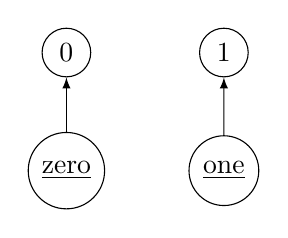
\begin{tikzpicture}[edge from parent/.style={draw,-latex}, align=center,node distance=2cm]

\node[circle,draw] (z){\underline{zero}} [grow = up]
    child{node [circle,draw]{0}
    };

\node[right of=z, circle,draw] {\underline{one}} [grow = up]
    child{node [circle,draw]{1}
    };

\end{tikzpicture}
\end{figure}

For each variable $x_i$ we construct a voter $x_i$ with voting profile $B_{x_i} = (  \text{\underline{zero}} > 1) $. We denote the primary preferences as full lines and the secondary preferences as dashed lines.

\begin{figure}[h]
    \centering
\begin{tikzpicture}[edge from parent/.style={draw,-latex}, align=center,node distance=2cm]

\node[circ] (x){$x_i$} [grow = up]

    child{node[circ] (1){1}  edge from parent [dashed]}
    child{node [circ] (z){\underline{zero}}{
        child{node[circ](0){0}}}
    };
\end{tikzpicture}
\end{figure}

We then construct gadgets for each term $t_h$. These gadgets will have the property that they incur no additional cost if $t_h$ is satisfied and a cost of at least one if $t_h$ is satisfied.

For a term $\overline{x_i} \lor x_j \lor x_k$: We construct additional voters $t_h$ and $a$, $b$ and $z$, with smart profiles:

\begin{align*}
    &B_z = (t_h > 0) \\
    &B_a = (x_i \land z> 0) \\
    &B_b = (x_j \lor a > 0) \\
    &B_{t_h} = (b \lor x_k > 0)
\end{align*}

This is demonstrated by the following figure:

\tikzset{circ/.style={circle,draw, solid, inner sep=0pt,minimum size=10mm}}
    \begin{figure}[h]
        \centering
    \begin{tikzpicture}[edge from parent/.style={draw,-latex}, align=center,node distance=1.75cm]
    
    \node[circ] (xi){$x_i$};
    \node[circ, right of=xi] (z){$z$};
    

    \node[circ, below of=xi] (xj){$x_j$};
    \node[circ, below of=xj] (xk){$x_k$};
    \node[circ, right of=xj] (a){$a$};
    \node[circ, right of=xk] (b){$b$};
    
    
    \node[draw, dashed, rounded rectangle, fit={(xi)(z)}] (elli1) {};
    \node[draw, dashed, rounded rectangle, fit={(a)(xj)}](elli2) {};
    \node[draw, dashed, rounded rectangle, fit={(b)(xk)}](elli3) {};

    \node[circ, below of=elli3](t){$t_h$};
    
    \draw [->] (a) -- (elli1) node[midway,left]{$\land$};
    \draw [->] (b) -- (elli2) node[midway,left]{$\lor$};
    \draw [->] (t) -- (elli3) node[midway,left]{$\lor$};
    \draw [->] (z.east) to [bend left=90] (t.east) {};
    
    \end{tikzpicture}
    \end{figure}
    
    Now, we analyse when first preferences of the additional voters can be resolved without producing cycles. If $x_k = 1$ then $t_h$ can resolve to $1$ and so will $z$. As $x_i$ and $z$ are set to a value $a$ can resolve its first preference. As $x_j$ and $a$ are set, $b$ can resolve its first delegation as well. Similarly if $x_j = 1$ then $b$ is immediately resolved to $1$ and so $t_h$ is resolved. Hence $z$ and then $a$ can be resolved. Similarly if $x_i = 0$ the logical AND of $a$ is resolved to $0$ and all additional voters are resolved.
    
    Now, suppose $x_i = 0, x_j = 0, x_k = 1$. Then $t_h$ cannot immediately resolve the logical OR as it is dependent on the vote of $b$, similarly $b$ is waiting for $a$ to decide, and $a$ is waiting for $z$. But $z$ is waiting for $t_h$ to decide. There is no way to resolve this cycle and so one of the additional voters we've introduced will have to vote for their second preference. This will incur an additional cost of at least 1.

    Now suppose that for each term we construct $n + 1$ such gadgets. Then if every term is satisfied by some assignment of the variables the maximum cost will be that of $n$. If a term is not satisfied then at least $n+1$ gadgets will incur a cost of $1$ so that the cost is at least $n+1$. Hence we have reduced the satisfiability of a \textsc{3-SAT} instance $\varphi$ to querying if there is a certificate $\vec{c}$ for the above election with $\sum_{i} \vec{c}_i \leq n$. Thus \textsc{BoundedMinSum}$_\mathcal{F}$ is NP-hard.
\end{proof}

\begin{corollary}[Inapproximability of \textsc{BoundedMinSum}] A constant factor approximation of \textsc{BoundedMinSum}$_\mathcal{F}$ is NP-hard.    
\end{corollary}

\begin{proof}
    We can adapt the above proof to prove that \textsc{BoundedMinSum} is not constant-factor approximable. Following our construction above we can incur a cost of $k$ for when the expression $\varphi$ is not satisfiable by simply creating $k$ gadgets for each term. So for a \textsc{MinSum} outcome $\vec{c}$:   $\sum_i \vec{c}_i \leq n$ if and only if $\varphi$ is satisfiable and $\sum_i \vec{c}_i \geq k$ if and only if $\varphi$ is not satisfiable. So, any constant factor approximator would solve \textsc{3-SAT}, thus proving hardness.
\end{proof}


\begin{proposition}[Hardness of \textsc{BoundedMinMax}]
    Suppose $\mathit{LIQUID} \cup \{\lor, \land\} \subseteq \mathcal{F}$. Then \textsc{BoundedMinMax} is NP-hard.    
\end{proposition}

\begin{proposition}[\textsc{BoundedMinMax} is not approximable]
    If $\mathit{LIQUID} \cup \{\lor, \land\} \subseteq \mathcal{F}$ then a non-trivial approximation of \textsc{BoundedMinMax} is NP-hard.
\end{proposition}

\newpage
\section{Axiomatisation}

We introduce the axiom of cast participation. That is that voters that have a preference for an outcome benefit from voting directly for it. We denote that agent $a$ prefers outcome $d$ to $e$ as $d >_a e$. We also infer that if agent $a$ votes directly for outcome $d$ then they weakly prefer $d$ over any other outcome. Formally if $B_a = (d)$ then for all $d' \in D$, $d \geq_a d'$.
Now, an issue is that irresolute unravelling procedures might return multiple outcomes. So \textsc{MinSum} can return outcomes for $0$ and for $1$.
So, we need to consider the set of outcomes from irresolute unravelling procedures. The simplest ordering of these sets of outcomes is that a voter $a$ that votes for $d$ prefers every set of outcomes that includes $d$ to every set of outcomes that doesn't. Further, $\{d\}$ is the preferred outcome of voter $a$. We assume that voters are indifferent between other sets of outcomes. 

Then we can formalise cast-participation for irresolute procedures:

\begin{definition}[Cast-Participation for irresolute procedures]
    A resolute voting rule $r$ and a irresolute unravelling procedure $\mathcal{U}$ satisfy cast-participation if for all valid smart profiles $\mathbf{B}$ and agents $a \in N$ such that $B_a \in D \setminus \{*\}$ we have that for all $B_a' \neq B_a$:
    \[
        r(\mathcal{U}(\mathbf{B})) \geq_a r(\mathcal{U}(\mathbf{B}_{-a}, B_a'))
    \]

    Where $\mathbf{B}_{-a}, B_a'$ denotes replacing $B_a$ with $B_a'$. 
\end{definition}

Cast participation can be thought of disallowing tactical voting. Unfortunatelly it does not always hold. 
We first prove the cases of non-monotone $r$ and non-monotone delegating functions. 
We prove these results for all unravelling procedures that would respect the voters first preference if the preferences didn't introduce cycles.

We now prove a series of negative results for cast participation.

\begin{lemma} Suppose $r$ is not monotone and $\mathcal{U}$ is any unravelling procedure, then cast participation doesn't hold.
\end{lemma}

\begin{proof}
    Suppose $r$ is not monotone. Then for some vector $\vec{u} \in D^n$ with $\vec{u}_i = 0$ there exists a $\vec{u}' = (\vec{u}_1, \ldots, \vec{u}_{i-1}, 1, \vec{u}_{i+1}, \ldots, \vec{u}_n )$ with $r(\vec{u}) = 1$ and $r(\vec{u}') = 0$. This violates cast participation by the following profile: let $B_a = (\vec{u}_a)$, so in particular voter $i$ prefers 0 to 1. Then voter $i$ strictly prefers to vote for 1 than 0. So, to achieve cast participation, $r$ must be monotone. 
\end{proof}

\begin{lemma}
    Suppose $r$ is a monotone rule, $\mathcal{U}$ respects first preferences and $f \in \mathcal{F}$ is a function on $D^k \longrightarrow D$ that is not monotone. Now suppose additionally that for some $n$ there exists a ``deciding'' subset of voters $S$ with $\abs{S} \leq n - k$ such that if every voter in $S$ votes for 0, $r$ votes for 0 and if every voter in $S$ votes for 1, $r$ votes for 1. Then cast-participation doesn't hold.
\end{lemma}

\begin{proof}
    Let $S$ and $f$ as defined above. Suppose $\vec{u} < \vec{u}'$ with only $\vec{u}_i \neq \vec{u}_i$ and $f(\vec{u}) > f(\vec{u}')$. Then, enumerate voters $v_1, \ldots, v_k$ not in $S$ and let $B_{v_i} = (\vec{u}_i)$. For all other agents $a$ set $B_{a} = (f(v_1, \ldots, v_k) > d)$ for some arbitrary $d$. 
    Then the first preferences of the voters do not introduce cycles. So
     $r$ resolves to vote for $1$ as all voters in $S$ vote for $1$.
    Now if $v_i$ were to switch their vote from $0$ to $1$ everyone in $S$ would vote for $0$ and so $r$ would resolve to $0$. This breaks cast participation for voter $v_i$.
\end{proof}

\begin{lemma}
    Let $r$ be a rule such that for $n \geq 5$ voters if $n-2$ voters vote for $d$ then $r$ assigns $d$. Let $\mathcal{F}$ contain LIQUID. Then there are examples that unravelling with \textsc{MinMax} violates cast-participation for any $n$.
\end{lemma}

\begin{proof}
    Let $N = \{v, v', a, u_1, \ldots, u_{n-3}\}$ and $r$ as described. Then, let $B_v = (0), B_{v'} = (v > 0), B_a = (1), B_{u_i} = (a > 0)$. Then \textsc{MinMax} would simply assign each individual to first preferences and the majority votes for 1. So the outcome set is $\{1\}$.

    But, if $B_v = (v' > 0)$ then a cycle is formed and so necessarily, \textsc{MinMax} will have to use some second preferences. Hence setting $v, u_1, \ldots, u_{n-3}$ to their second preference would be a valid solution. So every voter except $a$ vote for $0$, so that $r$ resolves to $0$. 
    Note that we can still assign first preference to all voters except than $v$ so that $(2, 1, \ldots, 1)$ is a consistent certificate and would result to the majority again voting for 1. So the set of outcomes is $\{0, 1\}$ which is better than $\{1\}$ for agent $a$.
\end{proof}

We can further prove that \textsc{MinSum} doesn't hold when using three symbols. To do this set $D = \{0, 1, *\}$ where $*$ denote abstentions.
In the case where abstentions are allowed we denote $\mathit{Maj}(0, *) = 0, \mathit{Maj}(1, *) = 1$ and $\mathit{Maj}(0, 1) = *$.

\begin{lemma}
    Let $D = \{0, 1, *\}$ and $r$ such that if a strict majority votes for outcome $d$ then $r$ supports outcome $d$. Let voters that directly vote for $0$ have preference $0 > * > 1$. Then if voters are allowed to delegate to even majorities, cast-participation doesn't hold for \textsc{MinSum}. 
\end{lemma}

\begin{proof}
    Let $N = \{a, b, c, d, e\}$. Let $B_a = (0), B_b = (1), B_c = (\mathit{Maj}(a, b) > 0), B_d = B_e = (c > 0)$. Then we can resolve this smart profile by assigning everyone to first preferences. Then $r$ delegates to $*$. So the set of outcomes is $\{*\}$.
    
    Now if $B_a' = (c > d > 0)$ then the unique result of \textsc{MinSum} is $c$ votes for $0$. Further, $a, d, e$ delegate to $c$ using first preferences and vote for $0$ as well. This results in a strict majority for $0$. So the set of outcomes is $\{0\}$ which is a preferred set of outcomes.
\end{proof}

Note, that in the above case $\mathit{Maj}$ is a monotone rule. So, it is not the case that monotone rules guarantee cast participation.

\iffalse
Plan for this section:
1) Cast participation is achieved only for monotone functions. So, let's focus on monotone functions
2) Prove NP-hardness for MinMax, MinSum using only binary or and binary and.
3) Prove that no constant approximator to MinMax or MinSum exists.
4) Result on whether we are able to even determine whether a vote is achievable.
5) Generalise on why the proof works for all non-delegative, fair and monotone functions. 
\fi

\newpage
\section{Proposals}

\end{document}

